\documentclass[a4paper,11pt]{article}
%Przydatne paczki:
\usepackage{amssymb}
\usepackage{amsthm}
\usepackage{amsmath}
\usepackage[colorinlistoftodos]{todonotes}
\usepackage[colorlinks=true, allcolors=blue]{hyperref}
%Definicja kodowania i języka:
\usepackage[polish]{babel}
\usepackage[MeX]{polski}
\usepackage[utf8]{inputenc}
\usepackage[T1]{fontenc}
%Paczki dodane w drodze pisania:
\usepackage{graphicx}
\usepackage{anysize}
\selectlanguage{polish}
\usepackage{tabularx}
\usepackage[export]{adjustbox}
\usepackage{listings}
\usepackage{float}
\usepackage{fancyhdr}

%Nagłówek:
\pagestyle{fancy}
\fancyhead{}
\fancyhead[L]{\small{\bfseries \thepage}}
\fancyfoot[L, C, R] {}
\fancyhead[C]{\small{\bfseries Dokumentacja projektu "Reflekto"}}
\renewcommand{\headrulewidth}{0.8pt}

%\marginsize{left}{right}{top}{bottom}
\marginsize{2.5cm}{2.5cm}{2.5cm}{2.5cm}

\begin{document}

\title{Dokumentacja projektu \\ \textbf{,,Reflekto'' } }
\author{Michał Kwiecień \\ Michał Wójcik}
%skomentować żeby nie było daty
%\date{\vspace{-5ex}}
\maketitle

\begin{abstract}
Dokumentacja projektu inteligentnego lustra w konwencji IoT komunikującego się ze smartfonem z użyciem interfejsu Bluetooth Low Energy. Projekt powstał na potrzeby konkursu Nordic Semiconductor Student Contest. 
\end{abstract}

\begin{figure}
	
\includegraphics[width=0.3\textwidth,center]{logo_nordic.png}
\end{figure}

\cleardoublepage
\tableofcontents
\clearpage

\section{Ogólny opis projektu}

Założeniem projektu jest stworzenie inteligentnego lustra, które podczas wykonywania codziennych czynności umożliwi podgląd najświeższych i spersonalizowanych informacji. Informacje te zostaną wyświetlone na wyświetlaczu umieszczonym za lustrem weneckim, dzięki czemu będą widoczne jednocześnie obok odbicia. 

Działanie lustra opiera się na przekazaniu danych poprzez moduł Bluetooth ze smartfona do modułu nRF52 i umieszczeniu ich na podłączonym ekranie. Aktywacja lustra nastąpi w momencie zbliżenia się do niego użytkownika. Z lustra może korzystać wielu użytkowników, gdyż każdorazowo przesyłane są indywidualne dane dla każdego z nich. 

W celu wygenerowania danych stworzona została dedykowana aplikacja dla systemu iOS. Po wstępnej konfiguracji umożliwi ona zautomatyzowanie procesu i przesyłanie wiadomości w tle bez późniejszych ingerencji użytkownika.


\section{Prezentacja działania}

Kiedy lustro nie jest w bliskim zasięgu jednego ze sparowanych telefonów, wyświetlana jest godzina lub pozostaje ono wyłączone w zależności od ustawień (Rys. \ref{lustro_off})

\begin{figure}[H]
	
\includegraphics[width=0.6\textwidth,center]{mirror_off.png}
	\caption {Lustro w stanie wyłączonym}
	\label{lustro_off}
\end{figure}

W momencie zbliżenia się użytkownika następuje transmisja danych i wyświetlenie aktualnych informacji (Rys. \ref{lustro_on}).

\begin{figure}[H]
	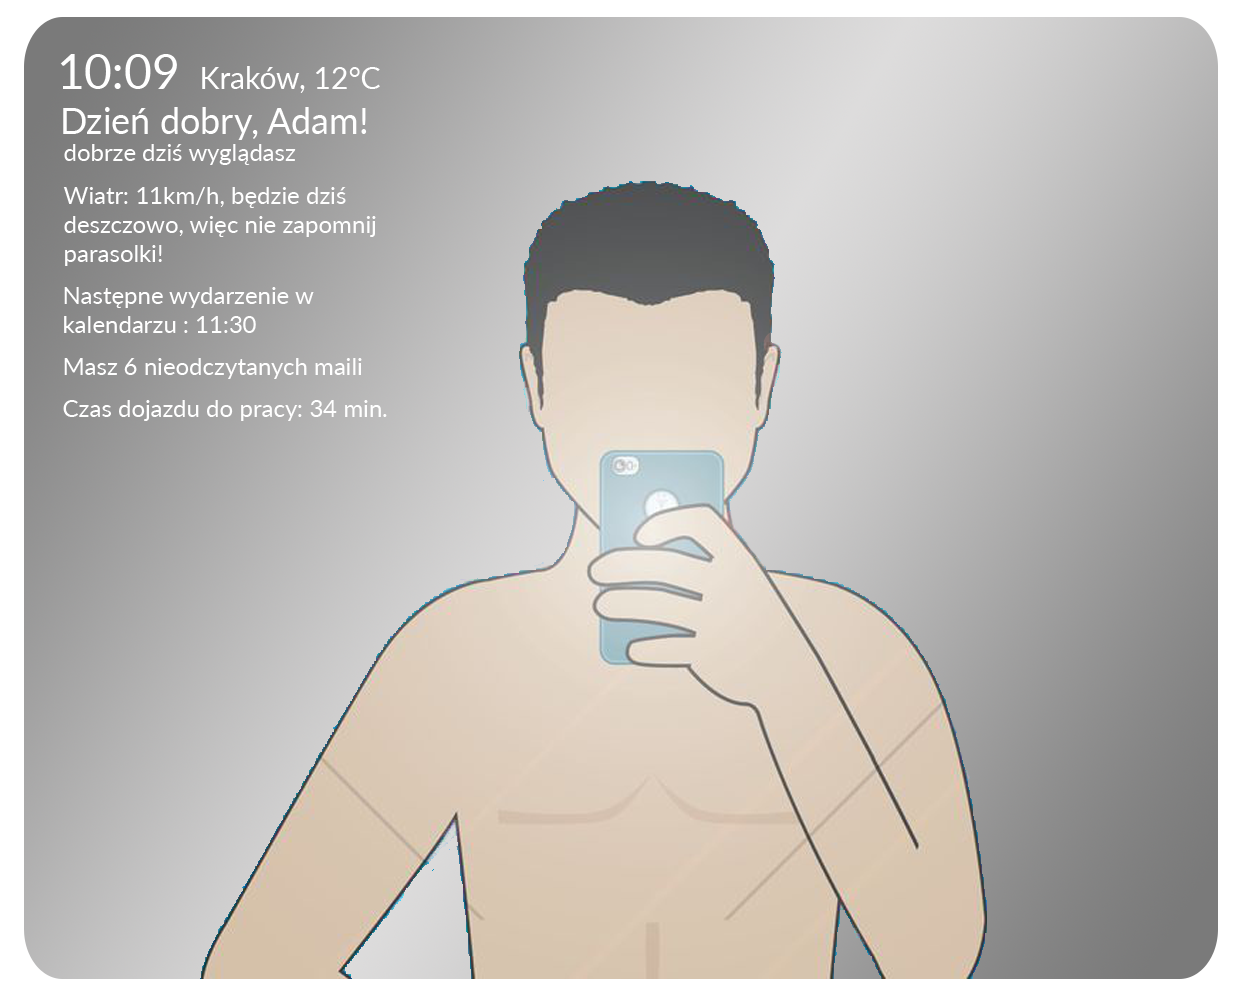
\includegraphics[width=0.6\textwidth,center]{mirror_on.png}
	\caption {Lustro w stanie aktywnym}
	\label{lustro_on}
\end{figure}

\section{Planowane możliwości personalizacji}
\begin{figure}[H]
	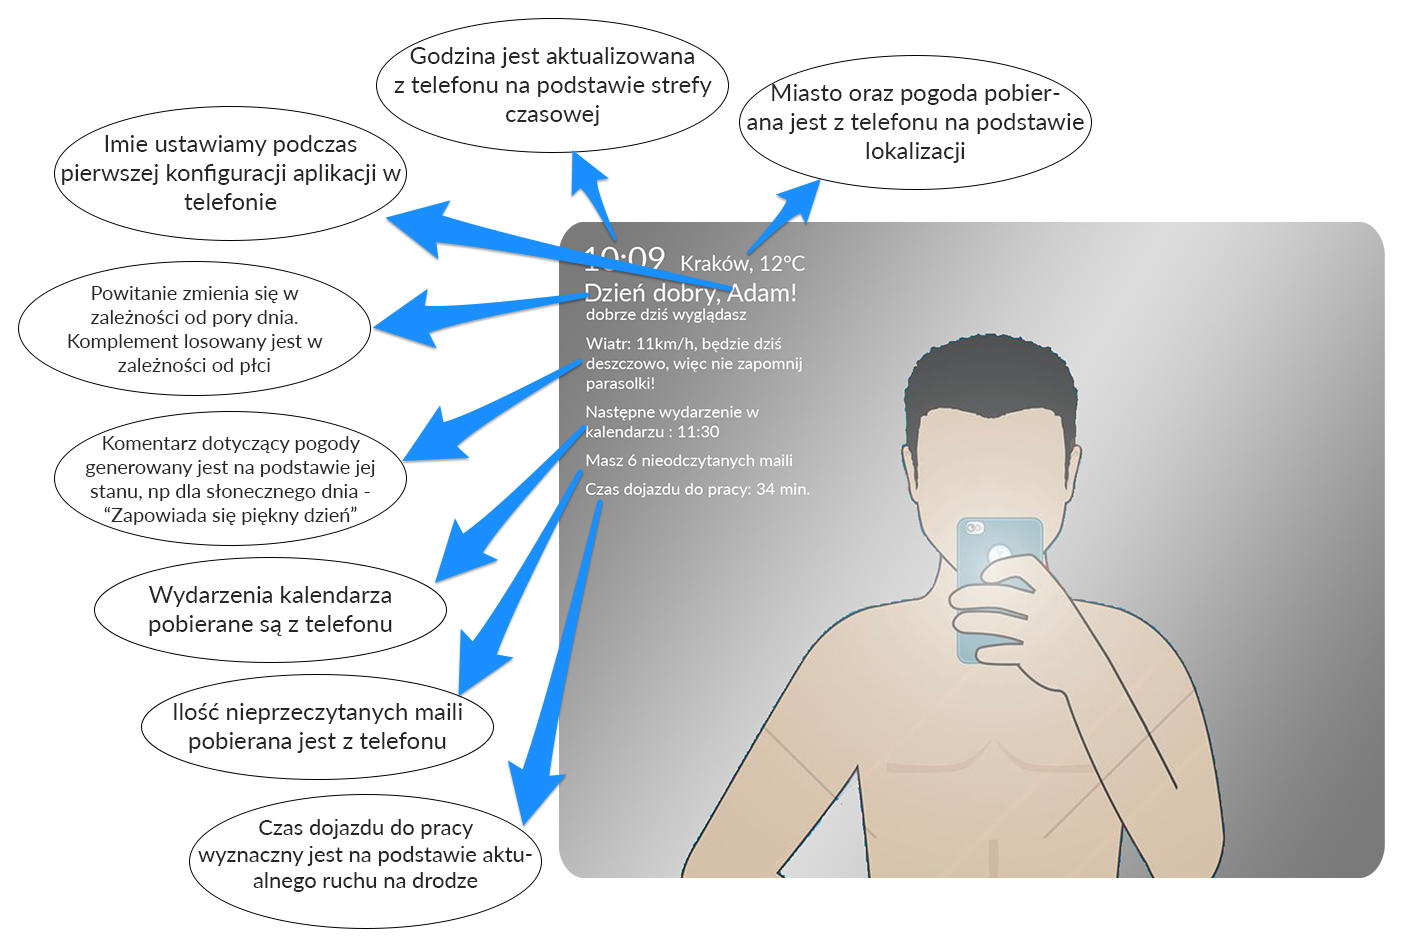
\includegraphics[width=0.9\textwidth,center]{dymki_kreski.png}
	\caption {Proponowane możliwości personalizacji}
	\label{lustro_konf}
\end{figure}

\section{Opis aplikacji systemu nRF52 (stan na 9 kwietnia 2017) }

\subsection{Włączenie urządzenia}
Urządzenie po uruchomieniu inicjalizuje wszystkie niezbędne usługi: timer, UART, stos BLE, serwisy oraz obsługę wyświetlacza. Dalej rozpoczyna się rozgłaszanie (pod nazwą ,,Reflekto\_UART'') i urządzenie pozostaje w stanie oczekiwania aż do wyłączenia zasilania. 

\subsection{Zasilanie}
Ze względu na użycie wyświetlacza TFT, wymagane jest zasilanie przez zasilacz zewnętrzny bądź port USB (bateria pastylkowa nie pokrywa zapotrzebowania na prąd). Obecnie szacowany pobór energii w stanie aktywnym wynosi mniej niż 900mW. W stanie nieaktywnym pobór energii przez wyświetlacz może zostać zredukowany do zera (sterowanie PWM), jednakże wymaga to wlutowania odpowiedniej zworki w płytkę wyświetlacza.

\subsection{Sposób rozgłaszania}
Do urządzenia w tym samym czasie może być podłączony jeden smartfon. W zależności od ustawień, 
 może być on połączony do momentu zachowania bliskiego zasięgu (potencjalnie blokując innych użytkowników), \todo{Możliwe korzystanie przez kilku użytkowników jednocześnie} lub rozłączać się od razu po przesłaniu informacji. 

Układ rozgłasza się pod wcześniej zdefiniowaną nazwą i UUID, udostępniając jeden serwis, z charakterystyką ,,write'' oraz ,notify'' (obecnie niewykorzystana).

\subsection{Realizacja komunikacji}
Układ w momencie otrzymania danych wysyła je do komputera przez port szeregowy (w celu debugowania), oraz rzutuje je na wektor typu \textit{char}, który przekazywany jest do kolejnej funkcji realizującej umieszczenie danych na wyświetlaczu.

Ze względu na ograniczenie ilości danych w pakiecie do 20 bajtów zastosowano specjalne kodowanie, gdzie pierwsze dwa bajty analizowane są w następujący sposób: 
\begin{itemize}
	\item bajt ,,0''
	\subitem Wskazuje na typ otrzymanych danych (np. data, godzina, pogoda, kalendarz, e-mali) \todo{4 bity można użyć do ,,szyfrowania'' transmisji}
	\item bajt ,,1''
	\subitem 4 bity górne -- numer aktualnie otrzymanego pakietu
	\subitem 4 bity dolne -- ilość wszystkich pakietów danego typu
\end{itemize}
Wynika z tego maksymalna długość przesyłanych danych jednego typu do 288 znaków (16 pakietów po 18 użytecznych bajtów). Podział na paczki realizowany jest przez aplikację na smartfonie. Założono także obsługę błędnych pakietów przez SoftDevice'a, dlatego nie uwzględnione zostały bajty na sumę CRC.

\subsection{Umieszczanie informacji na wyświetlaczu}
Po otrzymaniu wszystkich paczek danego typu, dane ,,drukowane'' są na wyświetlaczu (ze względu na metodę komunikacji niemożliwe jest przesłanie jednorazowo całej ramki obrazu). Wyświetlacz podzielony został na sekcje (od góry):
\begin{itemize}
	\item 20\% -- aktualna data i godzina
	\item 20\% -- aktualna pogoda
	\item 60\% -- kalendarz, czas dojazdu do pracy, emaile itd. wyświetlane cyklicznie bądź jednocześnie
\end{itemize}

\subsection{Planowany rozwój}
W planach jest obsługa danych konfiguracyjnych, które ustalałyby m.in. sposób wyświetlania informacji lub działania układu w trybie nieaktywnym. Dodatkowo w przypadku pomyślnego ukończenia projektu przed czasem, możliwe jest ponowne jego napisanie bez użycia protokołu UART, co zmniejszyłoby narzut na mikroprocesor.

\section{Opis aplikacji systemu iOS (stan na 9 kwietnia 2017)}

Aplikacja mobilna po uruchomieniu automatycznie rozpoznaje lokalizację użytkownika z dokładnością ok. 3km oraz próbuje nawiązać połączenie bluetooth z modułem lustra. Aktualny wygląd aplikacji pokazany jest obrazie (Rys. \ref{ios_main_screen})

\begin{figure}[H]
	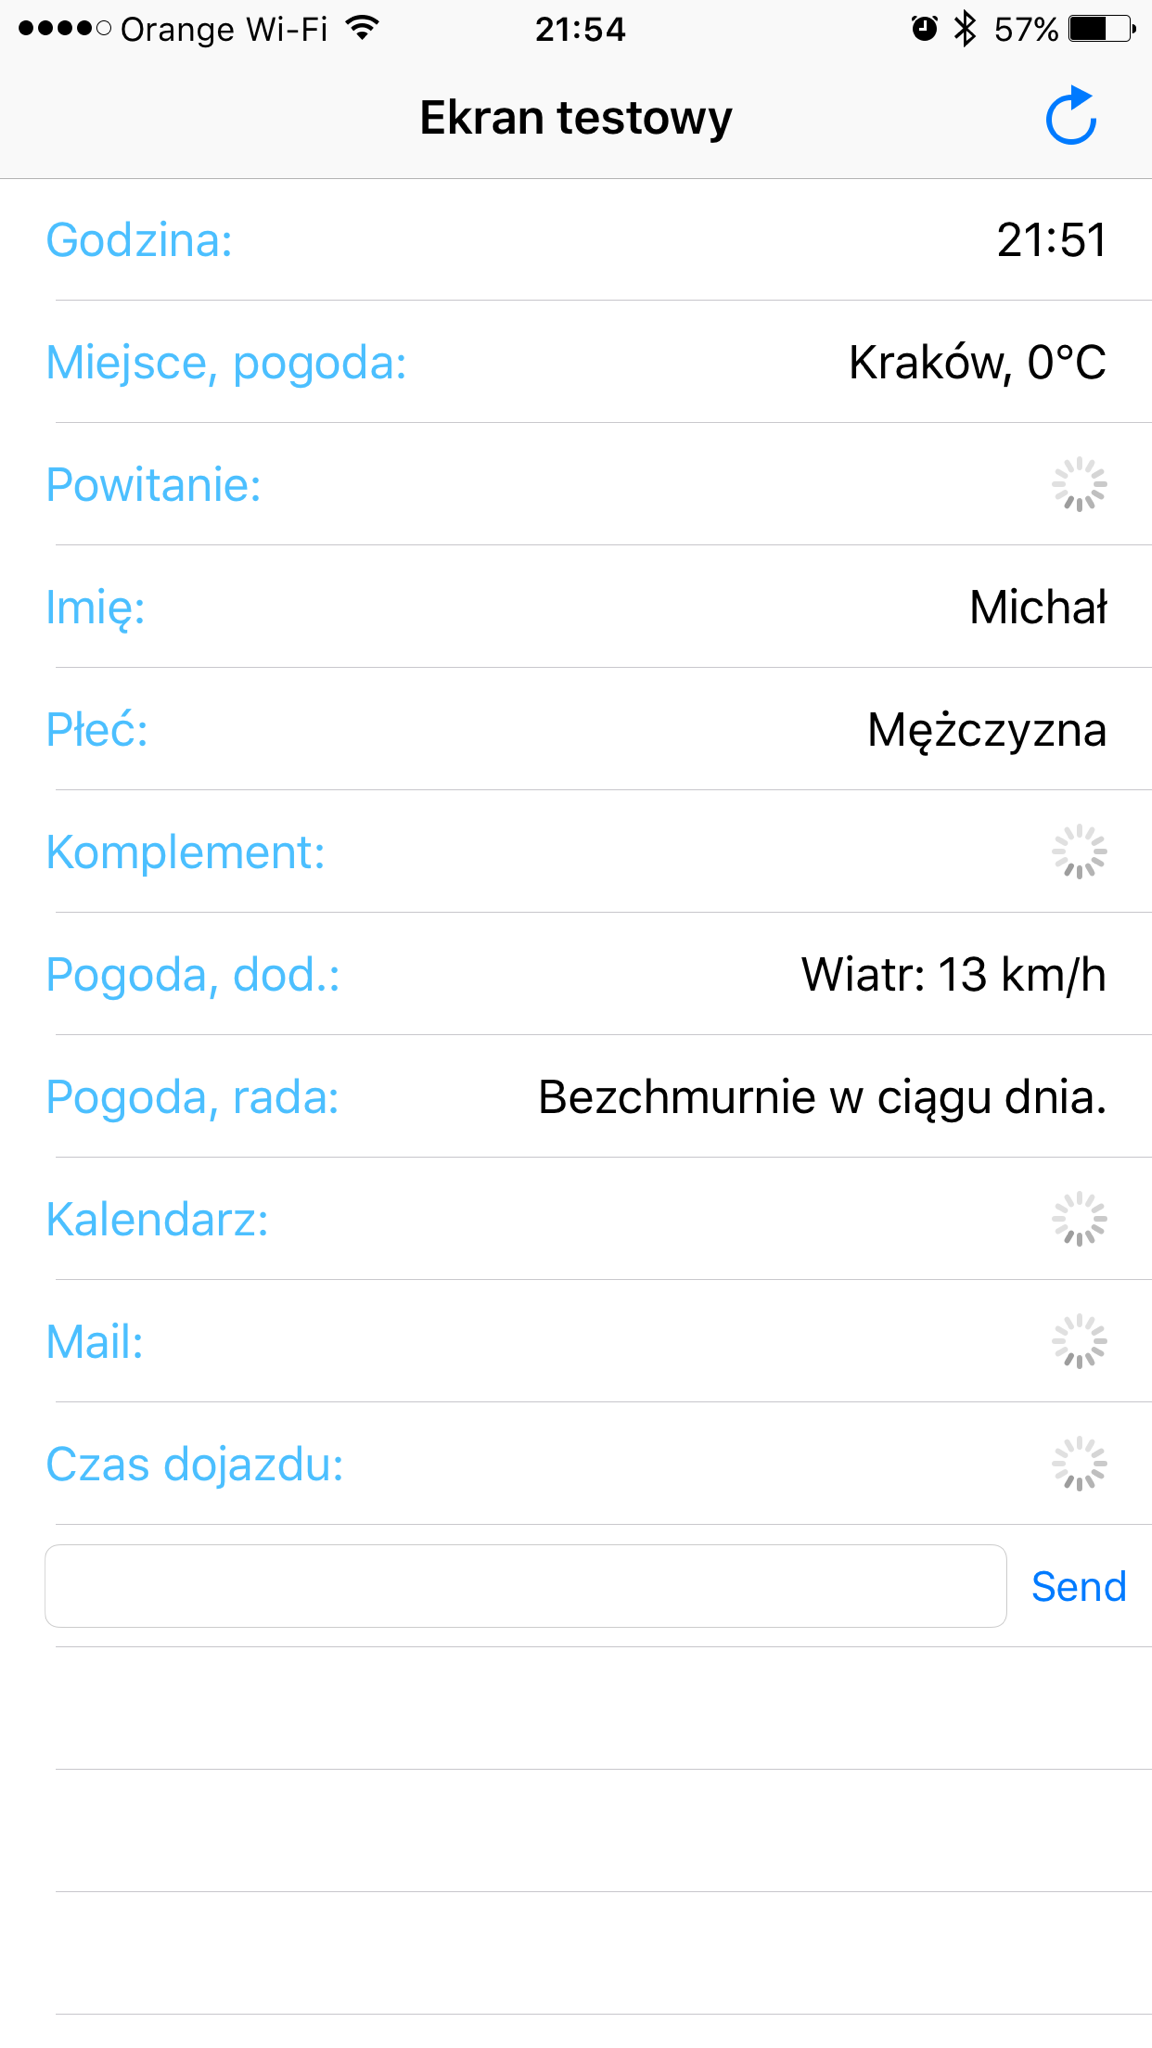
\includegraphics[width=0.4\textwidth,center]{ios_main_scrren.png}
	\caption {Aktualny wygląd aplikacji}
	\label{ios_main_screen}
\end{figure}

\subsection{Pobierane dane i sposób ich pobrania}
Aplikacja pobiera dane asynchronicznie, komórki z danymi w aplikacji uzupełniają się od razu po pobraniu poszczególnej danej. Nie trzeba czekać na zaktualizowanie interfejsu aż do momentu pobrania każdego elementu. Poniżej opis pobieranych danych oraz w przypadku bardziej złożonych informacji sposób ich pozyskania.

\begin{itemize}
	\item Godzina
	\item Miejsce, pogoda -- na podstawie wyznaczonej lokalizacji telefon wysyła zapytanie do Dark Sky API podając w parametrze m. in. długość oraz szerokość geograficzną. Otrzymany w odpowiedzi JSON parsowany jest na obiekt, z którego później wybierana jest temperatura. Miejsce wyznaczone jest również na podstawie szerokości i długości geograficznej używając wbudowanego  API Apple Maps.
	\item Imię -- imię użytkownika rozpoznawane jest automatycznie na podstawie nazwy urządzenia. Domyślnie ustawiona nazwa to np. ,,Michal's iPhone'' dla języka angielskiego lub ,,iPhone(Michał)'' dla języka polskiego. W przypadku innych wersji językowych nazwa urządzenia może być inna, więc metoda wykrywająca imię może nie zadziałać. Imię, które wykryjemy będzie jedynie propozycją podczas metody konfiguracji, jeśli użytkownik stwierdzi, że nie jest ono zgodne z prawdą będzie mógł je ręcznie wpisać.
	\item Płeć -- wyznaczana jest na podstawie ostatniej litery imienia, również będzie możliwa jej zmiana podczas procesu konfiguracji.
	\item Pogoda, dod. -- pobierana z Dark Sky API
	\item Pogoda, rada -- pobierana z Dark Sky API
\end{itemize}

\subsection{Sposób działania}
Po dotknięciu w poszczególną komórkę zostaje wygenerowany \textit{string} z dodanymi na początku dwoma bajtami, które pozwalają systemowi wbudowanemu zidentyfikować rodzaj informacji, która jest mu wysyłana. Po stworzeniu odpowiednich danych następuje próba wysłania informacji. Wykonywana jest na osobnym wątku, aby nie blokować interfejsu użytkownika.

W dolnej części interfejsu zostało dodane pole tekstowe ułatwiające proces przygotowania systemu wbudowanego. Można dzięki niemu wpisać dowolną informację, w jego przypadku nie są dodawane dodatkowe dwa bajty na początku.

\subsection{Planowany rozwój}

Aplikacja zostanie rozbudowana o proces konfiguracji, który użytkownik będzie musiał przejść tylko za pierwszym razem. Następne uruchomienia nie będą już wymagane, aplikacja będzie działać w tle i na podstawie skanera bluetooth uruchamiać się w pobliżu lustra. Dane będą dzielone na paczki i wysyłane do modułu bluetooth lustra.

Zostaną dodane kolejne dane pobierane z urządzenia, takie jak komplement generowany na podstawie płci lub informacje o nadchodzących wydarzeniach w kalendarzu.

Dodatkowo aplikacja zostanie przepisana, tak aby używała biblioteki RxSwift, która umożliwia pisanie kodu w sposób reaktywny i funkcjonalny. Do niektórych funkcji dodane zostaną również testy jednostkowe, oraz jeśli czas na to pozwoli integracja z systemem Travis w celu zastosowania continous integration.
	
	
\section{Podsumowanie}
	Projekt rozwijany jest z użyciem systemu kontroli wersji GitHub. Aktualne postępy dosępne są pod adresem: \url{https://github.com/Solstico}
	
	
	
	
	
	
\end{document}